% Options for packages loaded elsewhere
\PassOptionsToPackage{unicode}{hyperref}
\PassOptionsToPackage{hyphens}{url}
%
\documentclass[
]{article}
\usepackage{lmodern}
\usepackage{amssymb,amsmath}
\usepackage{ifxetex,ifluatex}
\ifnum 0\ifxetex 1\fi\ifluatex 1\fi=0 % if pdftex
  \usepackage[T1]{fontenc}
  \usepackage[utf8]{inputenc}
  \usepackage{textcomp} % provide euro and other symbols
\else % if luatex or xetex
  \usepackage{unicode-math}
  \defaultfontfeatures{Scale=MatchLowercase}
  \defaultfontfeatures[\rmfamily]{Ligatures=TeX,Scale=1}
\fi
% Use upquote if available, for straight quotes in verbatim environments
\IfFileExists{upquote.sty}{\usepackage{upquote}}{}
\IfFileExists{microtype.sty}{% use microtype if available
  \usepackage[]{microtype}
  \UseMicrotypeSet[protrusion]{basicmath} % disable protrusion for tt fonts
}{}
\makeatletter
\@ifundefined{KOMAClassName}{% if non-KOMA class
  \IfFileExists{parskip.sty}{%
    \usepackage{parskip}
  }{% else
    \setlength{\parindent}{0pt}
    \setlength{\parskip}{6pt plus 2pt minus 1pt}}
}{% if KOMA class
  \KOMAoptions{parskip=half}}
\makeatother
\usepackage{xcolor}
\IfFileExists{xurl.sty}{\usepackage{xurl}}{} % add URL line breaks if available
\IfFileExists{bookmark.sty}{\usepackage{bookmark}}{\usepackage{hyperref}}
\hypersetup{
  pdftitle={All Seasons Portfolio Part 2},
  pdfauthor={Stephen Lung},
  hidelinks,
  pdfcreator={LaTeX via pandoc}}
\urlstyle{same} % disable monospaced font for URLs
\usepackage[margin=1in]{geometry}
\usepackage{graphicx,grffile}
\makeatletter
\def\maxwidth{\ifdim\Gin@nat@width>\linewidth\linewidth\else\Gin@nat@width\fi}
\def\maxheight{\ifdim\Gin@nat@height>\textheight\textheight\else\Gin@nat@height\fi}
\makeatother
% Scale images if necessary, so that they will not overflow the page
% margins by default, and it is still possible to overwrite the defaults
% using explicit options in \includegraphics[width, height, ...]{}
\setkeys{Gin}{width=\maxwidth,height=\maxheight,keepaspectratio}
% Set default figure placement to htbp
\makeatletter
\def\fps@figure{htbp}
\makeatother
\setlength{\emergencystretch}{3em} % prevent overfull lines
\providecommand{\tightlist}{%
  \setlength{\itemsep}{0pt}\setlength{\parskip}{0pt}}
\setcounter{secnumdepth}{-\maxdimen} % remove section numbering

\title{All Seasons Portfolio Part 2}
\author{Stephen Lung}
\date{01-06-2020}

\begin{document}
\maketitle

\hypertarget{all-seasons-portfolio-part-2}{%
\section{All Seasons Portfolio Part
2}\label{all-seasons-portfolio-part-2}}

My third post to connect my learnings with my personal passion.

\hypertarget{business-science-problem-framework-bspf}{%
\section{Business Science Problem Framework
(BSPF)}\label{business-science-problem-framework-bspf}}

\begin{itemize}
\tightlist
\item
  With the increasing array of tools, I was swept away into some
  meaningless directions between advanced algorithms and other
  statistics. Therefofare I sat myself down to use a streamlined
  framework called the BSPF to re-orient myself. The BSPF is a
  systematic process to apply data science to business built on the
  learnings of Ray Dalio's philosophies in the book, Principles and
  Crisp DM
\end{itemize}

\begin{enumerate}
\def\labelenumi{\arabic{enumi}.}
\tightlist
\item
  How To Successfully Manage A Data Science Project: The Business
  Science Problem Framework from Matt Dancho's Business Science
  University
  (\url{https://www.business-science.io/business/2018/06/19/business-science-problem-framework.html})
  \textbackslash begin\{figure\}
\end{enumerate}

\{\centering 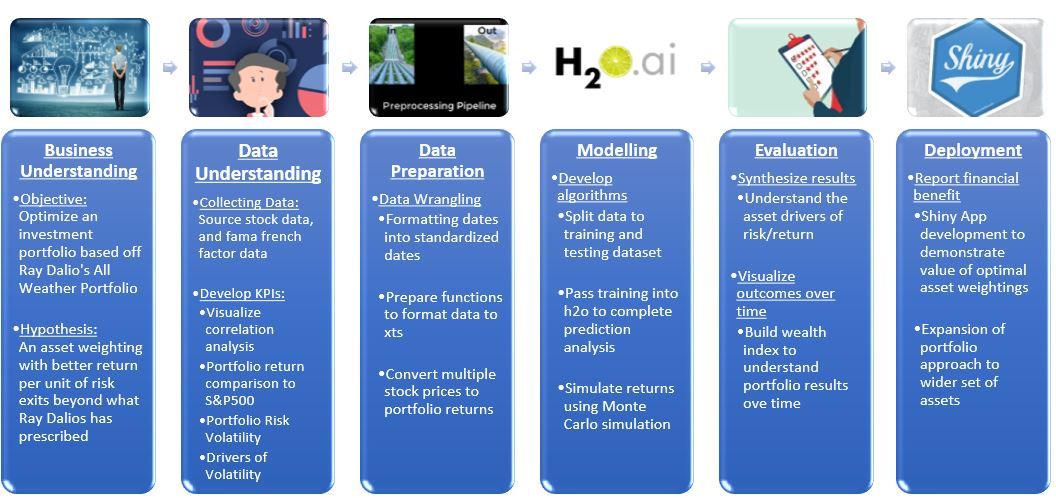
\includegraphics[width=1000px]{Images/Business Science Framework - V2}

\}

\caption{Business Science Problem Framework}\label{fig:unnamed-chunk-2}

\textbackslash end\{figure\}

\begin{enumerate}
\def\labelenumi{\arabic{enumi}.}
\setcounter{enumi}{1}
\tightlist
\item
  Principles by Ray Dalio (\url{https://www.principles.com/})
\end{enumerate}

\begin{figure}

{\centering 
\includegraphics[width=200px]{Images/Principles Ray Dalio} 

}

\caption{Principles}\label{fig:unnamed-chunk-3}
\end{figure}

\begin{enumerate}
\def\labelenumi{\arabic{enumi}.}
\setcounter{enumi}{2}
\tightlist
\item
  Reading the wealth of articles on Reproducible Finance with R: Code
  Flows and Shiny Apps for Portfolio Analysis by Jonathan K. Regenstein
  (\url{http://www.reproduciblefinance.com/})
  \textbackslash begin\{figure\}
\end{enumerate}

\{\centering 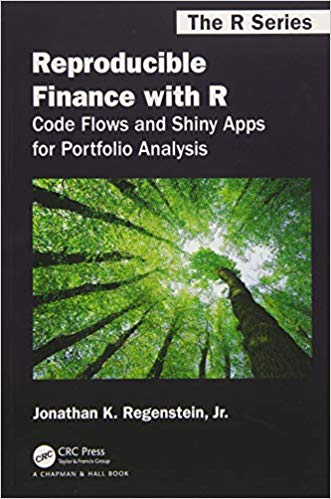
\includegraphics[width=200px]{Images/Reproducible Finance with R}

\}

\caption{Reproducible Finance with R: Code Flows and Shiny Apps for Portfolio Analysis}\label{fig:unnamed-chunk-4}

\textbackslash end\{figure\}

\emph{Credits go to both Matt Dancho and Jonathan K Regenstein in making
this post possible. Matt for educating me and creating the tidyquant
package and Jonathan for putting together a book for beginners.}

\hypertarget{business-understanding}{%
\section{Business Understanding}\label{business-understanding}}

\hypertarget{developing-a-portfolio-based-on-ray-dalios-all-weather-fund}{%
\subsection{Developing a Portfolio based on Ray Dalio's All Weather
Fund}\label{developing-a-portfolio-based-on-ray-dalios-all-weather-fund}}

In Tony Robbin's book - Master the Game, I learned about the All Weather
Fund and more about personal investing for the general public. Since
then I decided to complete a deeper dive on this portfolio and the
different asset classes to determine if data science can help me to
unlock some more financial benefits.

\textbf{Objective and Key Result}

\begin{itemize}
\item
  \textbf{Objective:} Optimize an investment portfolio based on Ray
  Dalio's All Weather Fund
\item
  \textbf{Hypothesis and Key Result:} An asset weighting with better
  return per unit of risk exists beyond what Ray Dalio has prescribed
\end{itemize}

\hypertarget{breakdown-of-all-weather-fund}{%
\subsection{Breakdown of All Weather
Fund}\label{breakdown-of-all-weather-fund}}

\begin{enumerate}
\def\labelenumi{\arabic{enumi}.}
\tightlist
\item
  40\% Long Term Bonds (TLT)
\item
  30\% Stocks (VTI)
\item
  15\% Intermediate Term Bonds (IEF)
\item
  7.5\% Gold (GLD)
\item
  7.5\% Commodities (DBC)
\end{enumerate}

\end{document}
